
\section{Full-dimensional checks of the reduced zero-mode model}\label{rep:v-fulldim}

The criterion of Secs.~\ref{rep:h-reduced}--\ref{rep:h-smmap} rests on a two-dimensional model of the Higgs zero mode, in which the Higgs radius $r$ and the length $s=|\bm w|$ of the hypercharge zero mode are dynamical and the nine SU(2) zero modes enter through a conditional Gaussian corrected by a fixed-$r$ diffusion Monte Carlo (DMC) shape term.
In this section we test that reduction against the full zero-mode problem with sixteen coordinates.
We find that, inside a gauge-invariant wall placed beyond the barrier, the full ground-state energy lies below the two-dimensional one at the same wall by $-0.0032(8)/L$ at $\lambda=-0.010$ and $-0.0034(9)/L$ at $\lambda=-0.013$, independently of the wall position and of $\lambda$ (it is $-0.0043(9)/L$ at $\lambda=0$). %
The reduction error is therefore a constant shift of the well.
Four independent estimates of the resulting change of the width give $\Gamma_{\rm full}/\Gamma_{\rm 2D}=0.92$--$1.03$. %
With the slopes of the final hazard this moves the critical top mass by $+0.0046$, $+0.0075$ and $+0.0115\GeV$ at $\Pone=0.9$, $0.5$ and $0.1$, with a one-sided envelope of $+0.012$, $+0.020$ and $+0.031\GeV$, which is the ``full-dimensional validation'' item of the error budget of Sec.~\ref{rep:h-budget}. %
The code and the archived outputs are in \texttt{higgs/05\_fulldim\_validation} of the code package~\cite{DNECv12code}; the derivation file is D123.

\subsection{The full zero-mode problem}\label{sec:v18-problem}

We use unit-mass coordinates $y=(\bm x,\bm w,\bm\phi)\in\mathbb R^9\times\mathbb R^3\times\mathbb R^4$: the constant SU(2) connections $x_i^a$ ($i$ spatial, $a$ adjoint), the constant hypercharge connections $w_i$, and the four real components of the Higgs zero mode, $\Phi=(\phi_0+i\phi_1,\phi_2+i\phi_3)/\sqrt2$, with $r=|\bm\phi|$ and $\Phi^\dagger\Phi=r^2/2$.
Lengths and energies are in units of the edge $L$ (Sec.~\ref{rep:setup}).
The Hamiltonian is
\begin{equation}
H=\tfrac12\,p^2+V(y),
\label{eq:v18-H}
\end{equation}
with
\begin{equation}
V(y)=g_2^2\,v_{\rm su2}(\bm x)+\sum_{i=1}^3\bigl|\bigl(g_2\,x_i^aT^a+g_Y\,Y\,w_i\bigr)\Phi\bigr|^2+\frac{\lambda}{4}\,r^4+\Delta V_{\rm MC}(r),
\label{eq:v18-V}
\end{equation}
where $T^a=\sigma^a/2$, $Y=1/2$, and
\begin{equation}
v_{\rm su2}(\bm x)=\frac14\sum_{i,j=1}^{3}\bigl|\bm x_i\times\bm x_j\bigr|^2
\label{eq:v18-vsu2}
\end{equation}
is the magnetic energy of constant SU(2) connections, $\bm x_i$ being the adjoint three-vector of direction $i$.
The last term of Eq.~(\ref{eq:v18-V}) is the one-loop matching of the non-zero modes of Sec.~\ref{rep:h-matching} (Coulomb gauge with the $\MSbar$ finite-volume sums), which depends on $r$ only; we evaluate it on $0\le r\le r_w$ with step $0.002$ and interpolate with a cubic spline.
All numbers in this section use the one-loop couplings of the zero-mode calculation of Sec.~\ref{rep:zeromodes}, $g_2=0.5268$, $g_Y=0.4415$ and $y_t=0.4585$, the second-stage model without the cross terms of Sec.~\ref{rep:h-cross}, and the full width $\Gamma=-2\,{\rm Im}\,E$ in units of $1/L$. %

For $\lambda<0$ the potential is unbounded from below along $r$, and the Hamiltonian~(\ref{eq:v18-H}) has no ground state; the resonance of Sec.~\ref{rep:h-reduced} is a Siegert state.
To obtain a ground-state problem that DMC can solve we impose a Dirichlet wall at $|\bm\phi|=r_w$.
Three properties make this wall harmless.
\begin{enumerate}
\item Constant SU(2)$\times$U(1)$_Y$ transformations act on $(\bm x,\bm w,\bm\phi)$ by orthogonal matrices and preserve $|\bm\phi|$, so both the wall and $H$ are gauge invariant.
\item The region $\{|\bm\phi|<r_w\}\times\mathbb R^{12}$ is connected and the Dirichlet semigroup $e^{-tH}$ is positivity improving on it.
The ground state is therefore unique and positive, hence invariant under every symmetry of $H$; in particular it is gauge invariant and satisfies Gauss's law without a projection.
\item The wall is the only node of the ground state, and it is exact.
DMC with a guiding function that vanishes on the wall therefore has no fixed-node error.
\end{enumerate}
Inside the wall the quartic term is bounded, $|\lambda| r^4/4\le|\lambda| r_w^4/4$, and the walled ground state exists.

\subsection{Placement of the walls}\label{sec:v18-walls}

We place the walls with the lowest adiabatic channel of the two-dimensional model,
\begin{equation}
U_{\rm ad}(r)=U_1(r)+\tfrac32\,\Omega_{\rm eff}(r),
\label{eq:v18-Uad}
\end{equation}
where $U_1$ is the $r$-dependent part of the two-dimensional Hamiltonian and $\Omega_{\rm eff}$ the stiffness of $\bm w$ (Sec.~\ref{rep:h-reduced}).
Let $r_1$ and $r_2$ be the inner and outer classical turning points at the resonance energy $\varepsilon$ and $r_{\rm top}$ the position of the barrier top.
A wall with $r_{\rm top}<r_w<r_2$ leaves no classically allowed region below $\varepsilon$ outside the barrier, so the lowest walled state is the state localized in the well.
Table~\ref{tab:v18-walls} lists the geometry and the walls.
Two further walls inside the barrier top serve only the tail estimate of Sec.~\ref{sec:v18-tail}.

\begin{table}[t]
\centering
\caption{Geometry of the lowest adiabatic channel~(\ref{eq:v18-Uad}) and positions of the walls (units of $L$). $U_{\rm ad}(r_w)-\varepsilon$ is given for the three main walls. Two inner walls, used only for the tail estimate, lie at $4.08$ and $4.32$ ($\lambda=-0.010$) and at $3.84$ and $4.08$ ($\lambda=-0.013$).}
\label{tab:v18-walls}
\begin{tabular}{ccccccc}
\toprule
$\lambda$ & $r_1$ & $r_{\rm top}$ & $U_{\rm top}$ & $r_2$ & main walls $r_w$ & $U_{\rm ad}(r_w)-\varepsilon$ \\
\midrule
$-0.010$ & $2.498$ & $4.344$ & $5.002$ & $5.737$ & $4.80,\ 5.12,\ 5.44$ & $0.64,\ 0.51,\ 0.26$ \\ %
$-0.013$ & $2.510$ & $4.022$ & $4.812$ & $5.188$ & $4.40,\ 4.64,\ 4.96$ & $0.48,\ 0.38,\ 0.17$ \\ %
\bottomrule
\end{tabular}
\end{table}

\begin{figure}[t]
\centering
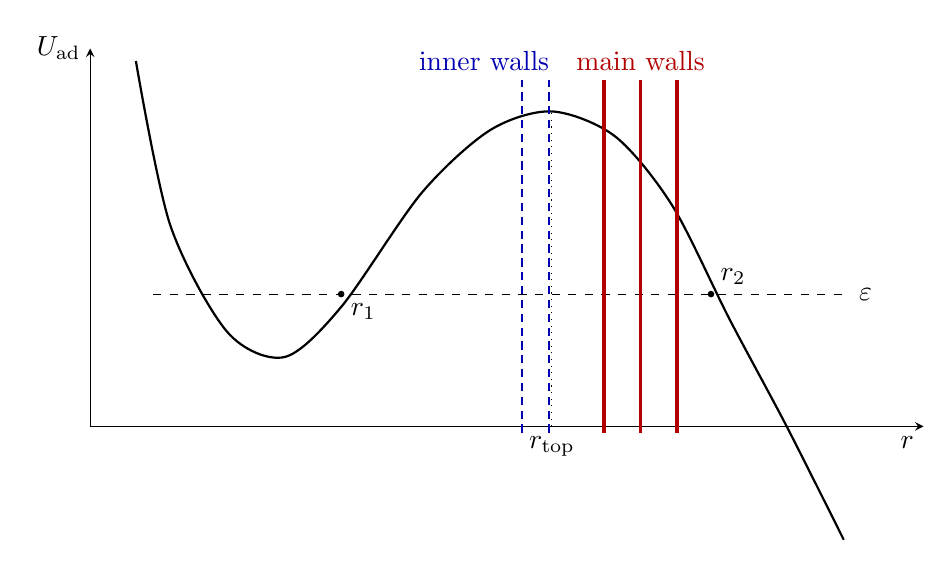
\begin{tikzpicture}[x=1.45cm,y=1.6cm,>=stealth]
\draw[->] (0.3,0) -- (7.6,0) node[below left]{$r$};
\draw[->] (0.3,0) -- (0.3,3.0) node[left]{$U_{\rm ad}$};
\draw[thick,smooth] plot coordinates {(0.7,2.9) (1.0,1.6) (1.5,0.75) (2.0,0.55) (2.5,0.95) (3.2,1.85) (3.8,2.35) (4.344,2.5) (4.9,2.3) (5.4,1.75) (5.9,0.85) (6.4,0.0) (6.9,-0.9)};
\draw[dashed] (0.85,1.05) -- (6.95,1.05) node[right]{$\varepsilon$};
\fill (2.498,1.05) circle (1.2pt) node[below right]{$r_1$};
\fill (5.737,1.05) circle (1.2pt) node[above right]{$r_2$};
\draw[dotted] (4.344,0) -- (4.344,2.5);
\node[below] at (4.344,0) {$r_{\rm top}$};
\foreach \x in {4.80,5.12,5.44} \draw[very thick,red!70!black] (\x,-0.05) -- (\x,2.75);
\foreach \x in {4.08,4.32} \draw[thick,blue!70!black,densely dashed] (\x,-0.05) -- (\x,2.75);
\node[red!70!black,above] at (5.12,2.75) {main walls};
\node[blue!70!black,above] at (3.75,2.75) {inner walls};
\end{tikzpicture}
\caption{Schematic of the walled problem at $\lambda=-0.010$ (not to scale). The main walls (solid) lie between the barrier top $r_{\rm top}=4.344$ and the outer turning point $r_2=5.737$ of the lowest adiabatic channel, so the lowest walled state is the well state; the inner walls (dashed), inside the barrier top, shift the energy by an amount set by the tunnelling tail and are used only for the tail-amplitude estimate of Sec.~\ref{sec:v18-tail}.}
\label{fig:v18-walls}
\end{figure}

\subsection{Diffusion Monte Carlo inside the wall}\label{sec:v18-dmc}

DMC projects the ground state by evolving in imaginary time.
For a guiding function $\psi_T$ and the mixed density $f(y,t)=\psi_T(y)\,\psi(y,t)$ the imaginary-time Schr\"odinger equation $-\partial_t\psi=(H-E_{\rm ref})\psi$ becomes
\begin{equation}
-\partial_t f=-\tfrac12\nabla^2f+\nabla\cdot\bigl(f\,\bm v\bigr)+\bigl[E_L(y)-E_{\rm ref}\bigr]f,
\qquad
\bm v=\nabla\ln\psi_T,\qquad E_L=\frac{H\psi_T}{\psi_T},
\label{eq:v18-fp}
\end{equation}
a drift--diffusion equation with branching~\cite{Foulkes:2001zz,Kosztin:1996fh}.
As $t\to\infty$, $f\to\psi_T\psi_0$, and the mixed estimator
\begin{equation}
E_{\rm mix}=\frac{\int f\,E_L\,dy}{\int f\,dy}=\frac{\langle\psi_0|H|\psi_T\rangle}{\langle\psi_0|\psi_T\rangle}=E_0
\label{eq:v18-mixed}
\end{equation}
is exact, because $H$ is Hermitian on functions that vanish on the wall and $\psi_0$ and $\psi_T$ obey the same Dirichlet condition.

\paragraph{Guiding function.}
We use
\begin{equation}
\psi_T(y)=\exp\!\Bigl(-\tfrac12a_x|\bm x|^2-\tfrac12a_w|\bm w|^2\Bigr)\,f_r(r),
\label{eq:v18-psiT}
\end{equation}
with $(a_x,a_w)$ from the optimal Gaussian at $\lambda=0$ of the zero-mode calculation and $f_r$ the ground state of the radial problem
\begin{equation}
-\frac12\Bigl(f_r''+\frac3r\,f_r'\Bigr)+U_g(r)\,f_r=\epsilon\,f_r,\qquad f_r(r_w)=0,
\label{eq:v18-radial}
\end{equation}
where $U_g=\frac\lambda4r^4+\Delta V_{\rm MC}+C_0+B_x+\delta E_{\rm DMC}+\frac32\Omega_{\rm eff}$ is the lowest adiabatic channel of the two-dimensional model without the Born--Huang term $B_w$ (Sec.~\ref{rep:h-reduced}); the factor $3/r$ is the radial Laplacian of the four Higgs components.
We solve Eq.~(\ref{eq:v18-radial}) by finite differences with step $0.001$ and interpolate $f_r$ by a cubic spline with $f_r'(0)=0$.
The local energy follows directly from the spline,
\begin{equation}
E_L(y)=\frac12\sum_ia_i-\frac12\sum_ia_i^2y_i^2-\frac{f_r''+3f_r'/r}{2f_r}+V(y),
\label{eq:v18-EL}
\end{equation}
where the sums run over the twelve gauge coordinates with $a_i=a_x$ or $a_w$; it is evaluated from the same spline that drives the walkers, so the drift, the Metropolis ratio and $E_L$ are consistent.

\paragraph{Moves and population.}
Each walker moves by the short-time Green function $y'=y+\bar{\bm v}\,\tau+\sqrt\tau\,\bm\eta$, $\bm\eta$ a standard normal vector, and the move is accepted with the Reynolds--Umrigar Metropolis probability that restores detailed balance for $\psi_T^2$~\cite{Umrigar:1993dmc}.
On the four Higgs components the drift is limited as
\begin{equation}
\bar{\bm v}=\frac{-1+\sqrt{1+2a\,v^2\tau}}{a\,v^2\tau}\;\bm v,\qquad a=0.5,
\label{eq:v18-drift}
\end{equation}
which leaves small drifts unchanged and caps the drift near the node at the wall; the same formula is used in the forward and the reverse Green function. %
Every proposal with $r'\ge r_w$ is rejected, since $\psi_T=0$ there; at most $2\times10^{-6}$ of the moves are rejected for this reason. %
Branching uses the effective time step $\tau_{\rm eff}=\tau\times(\text{acceptance ratio})$, the population is fixed at $W=10^4$ walkers by systematic resampling, and $E_{\rm ref}$ is adjusted slowly. %

\paragraph{Statistics and time step.}
For every wall and every time step we run two independent shards, each with equilibration time $10$ and production time $40$.
The seed of a shard is fixed by the SHA-256 hash of the string \texttt{T14a|name|tau|k} and recorded in its output, so that each shard can be rerun bit for bit (the package rerun of one shard is identical).
Errors are block averages, the largest over block lengths $1$, $2$ and $4$; shards are combined with inverse-variance weights and the error is inflated when their scatter exceeds it.
We extrapolate linearly in $\tau_{\rm eff}$ from $\tau=0.04$, $0.02$ and $0.01$; the fitted slopes are $0.02$--$0.15$ with $\chi^2\le1.6$ for one degree of freedom, and the extrapolated energy differs from the smallest-step value by at most $0.002$, which is contained in the extrapolation error. %
After extrapolation the statistical error of a single wall is $0.0010$--$0.0025$. %
In total the calculation uses $66$ shards (eleven walled cases, three time steps, two shards each).

\subsection{The two-dimensional model at the same wall}\label{sec:v18-2d}

The comparison must use the same wall in both models, because a wall below the barrier top shifts the two-dimensional energy by up to $0.024$, far more than the effect we look for.
We discretize the two-dimensional Hamiltonian of Sec.~\ref{rep:h-reduced} (both the model with the DMC shape correction, 2D, and its Gaussian version, 2D$_{\rm G}$) with second-order finite differences in $r$ and $s$, with Dirichlet conditions at $r=r_w$ and $s=12$, at steps $h=0.08$, $0.04$ and $0.02$.
For an energy $E(h)=E+c_2h^2+c_4h^4+O(h^6)$ the two Richardson steps
\begin{equation}
E^{(2)}(h)=\frac{4E(h/2)-E(h)}{3},\qquad E^{(4)}=\frac{16E^{(2)}(h/2)-E^{(2)}(h)}{15}
\label{eq:v18-richardson}
\end{equation}
remove the $h^2$ and $h^4$ terms; $E^{(2)}$ and $E^{(4)}$ differ by at most $2\times10^{-6}$. %
At $\lambda=0$ the code reproduces the finite-difference values $4.450855$ (2D) and $4.507693$ (2D$_{\rm G}$) of the reduced-model calculation, which the Numerov solver of Sec.~\ref{rep:h-reduced} gives as $4.450863$. %
A $\pm1\sigma$ tilt of the DMC shape correction $\delta E_{\rm DMC}$ changes the two-dimensional energy by $\pm0.0025$ at $\lambda=0$ and $\pm0.0022$ at the middle walls for $\lambda<0$. %
The full DMC contains no such correction, so the difference $\Delta\varepsilon=\varepsilon_{\rm full}-\varepsilon_{\rm 2D}$ measures the reduction error relative to the central two-dimensional model.

\subsection{Results}\label{sec:v18-results}

\paragraph{The benchmark at $\lambda=0$.}
Table~\ref{tab:v18-lam0} compares the reductions of the zero-mode problem with the full-dimensional DMC value at $\lambda=0$, $4.4478(13)$, without the matching term. %
The two-dimensional model is the only reduction within $0.004$ of the full value; the one-dimensional Gaussian reduction is $0.151$ too high, and the two Born--Oppenheimer bounds bracket the full value at $-0.014$ and $+0.098$.

\begin{table}[t]
\centering
\caption{Ground-state energy at $\lambda=0$ (units of $1/L$; local model without the matching term) for the reductions of Sec.~\ref{rep:h-reduced}, compared with full-dimensional DMC, $4.4478(13)$.}
\label{tab:v18-lam0}
\begin{tabular}{lcc}
\toprule
Reduction & $L\varepsilon_0$ & Difference \\
\midrule
One-dimensional, Gaussian (with $B_r$) & $4.5985$ & $+0.151$ \\ %
One-dimensional, exact gauge shape & $4.5434$ & $+0.096$ \\ %
Born--Oppenheimer bound, with $B_w$ & $4.5462$ & $+0.098$ \\ %
Born--Oppenheimer bound, without $B_w$ & $4.4334$ & $-0.014$ \\ %
Two-dimensional, Gaussian (2D$_{\rm G}$) & $4.5077$ & $+0.060$ \\ %
Two-dimensional (2D) & $4.4509$ & $+0.0031$ \\ %
\quad without $B_x$ & $4.4456$ & $-0.0022$ \\ %
\bottomrule
\end{tabular}
\end{table}

The walled code of this section, with the wall at $r_w=9$ where it has no effect, gives
\begin{equation}
\varepsilon_{\rm full}(\lambda=0)=4.44659(94),
\label{eq:v18-lam0}
\end{equation}
with a time-step slope of $0.083$ and $\chi^2=0.14$ for one degree of freedom. %
The unwalled code of the zero-mode calculation gives $4.44781(132)$; the difference is $-0.0012(16)$, or $0.75\sigma$, and the combined value is $4.44700(77)$. %
Against the two-dimensional model at the same wall ($r_w=8.96$), $\Delta\varepsilon(\lambda=0)=-0.0043(9)$, or $-0.0039(8)$ with the combined value; against 2D$_{\rm G}$ it is $-0.0611$. %

\paragraph{Negative quartic coupling.}
Tables~\ref{tab:v18-m010} and~\ref{tab:v18-m013} give the energies at every wall.
The Siegert resonance of the two-dimensional model lies at $\varepsilon_{\rm 2D}=4.286744$ with $\Gamma_{\rm 2D}=4.1535\times10^{-4}$ for $\lambda=-0.010$, and at $4.277899$ with $\Gamma_{\rm 2D}=2.2162\times10^{-3}$ for $\lambda=-0.013$; the column ``2D wall shift'' is the difference between the walled two-dimensional energy and this Siegert value. %

\begin{table}[t]
\centering
\caption{Walled energies at $\lambda=-0.010$ (units of $1/L$): full-dimensional DMC (extrapolated to zero time step), the two-dimensional model 2D and its Gaussian version 2D$_{\rm G}$ at the same wall (finite differences with Richardson extrapolation), their difference $\Delta\varepsilon=\varepsilon_{\rm full}-\varepsilon_{\rm 2D}$, and the shift of the 2D energy by the wall. The first two walls lie inside the barrier top.}
\label{tab:v18-m010}
\begin{tabular}{cccccc}
\toprule
$r_w$ & $\varepsilon_{\rm full}$ & $\varepsilon_{\rm 2D}$ & $\Delta\varepsilon$ & $\varepsilon_{\rm 2D_G}$ & 2D wall shift \\
\midrule
$4.08$ & $4.29394(145)$ & $4.298235$ & $-0.0043(15)$ & $4.352733$ & $+0.0115$ \\ %
$4.32$ & $4.29005(96)$ & $4.293356$ & $-0.0033(10)$ & $4.347474$ & $+0.0066$ \\ %
$4.80$ & $4.28584(103)$ & $4.288989$ & $-0.0031(10)$ & $4.342681$ & $+0.0022$ \\ %
$5.12$ & $4.28451(145)$ & $4.287887$ & $-0.0034(14)$ & $4.341440$ & $+0.0011$ \\ %
$5.44$ & $4.28411(203)$ & $4.287352$ & $-0.0032(20)$ & $4.340824$ & $+0.0006$ \\ %
\bottomrule
\end{tabular}
\end{table}

\begin{table}[t]
\centering
\caption{As Table~\ref{tab:v18-m010}, at $\lambda=-0.013$. The first two walls lie inside the barrier top.}
\label{tab:v18-m013}
\begin{tabular}{cccccc}
\toprule
$r_w$ & $\varepsilon_{\rm full}$ & $\varepsilon_{\rm 2D}$ & $\Delta\varepsilon$ & $\varepsilon_{\rm 2D_G}$ & 2D wall shift \\
\midrule
$3.84$ & $4.29921(117)$ & $4.302053$ & $-0.0028(12)$ & $4.356919$ & $+0.0242$ \\ %
$4.08$ & $4.29064(105)$ & $4.292774$ & $-0.0021(10)$ & $4.347034$ & $+0.0149$ \\ %
$4.40$ & $4.28018(252)$ & $4.285813$ & $-0.0056(25)$ & $4.339513$ & $+0.0079$ \\ %
$4.64$ & $4.27915(144)$ & $4.282919$ & $-0.0038(14)$ & $4.336333$ & $+0.0050$ \\ %
$4.96$ & $4.27798(118)$ & $4.280700$ & $-0.0027(12)$ & $4.333852$ & $+0.0028$ \\ %
\bottomrule
\end{tabular}
\end{table}

The inverse-variance means over the three main walls are
\begin{equation}
\Delta\varepsilon(-0.010)=-0.00323(78),\qquad \Delta\varepsilon(-0.013)=-0.00343(86),
\label{eq:v18-dE}
\end{equation}
with $\chi^2=0.02$ and $1.2$ for two degrees of freedom. %
Three facts follow from the tables.
First, $\Delta\varepsilon$ does not depend on the wall, although the two-dimensional wall shift itself varies from $0.0006$ to $0.008$ over the main walls and up to $0.024$ over all walls; the effect of the wall cancels in the difference.
The inner walls agree within errors (at $\lambda=-0.013$ the innermost two are slightly smaller, $-0.0028(12)$ and $-0.0021(10)$), and there is no trend with $r_w$.
Second, $\Delta\varepsilon$ does not depend on $\lambda$: $-0.0043(9)$, $-0.0032(8)$ and $-0.0034(9)$ at $\lambda=0$, $-0.010$ and $-0.013$.
The reduction error is a constant shift of about $-0.0035/L$ of the well.
Third, $\varepsilon_{\rm full}<\varepsilon_{\rm 2D_G}$ by $0.057$ at both negative couplings, so the variational bound of the Gaussian model, an upper bound for the trial family of Sec.~\ref{rep:h-reduced}, holds with the wall as well. %
The target $|\Delta\varepsilon|\le0.005$ set before the calculation is met at the central values; the $2\sigma$ upper limits are $0.0048$ and $0.0051$. %

\subsection{From the energy shift to the width: four estimates}\label{sec:v18-gamma}

A shift of the well changes the width through the energy at which the particle meets the barrier.
If the barrier is unchanged,
\begin{equation}
\rho\equiv\frac{\Gamma_{\rm full}}{\Gamma_{\rm 2D}}=\exp\!\Bigl(\Delta\varepsilon\,\frac{d\ln\Gamma}{d\varepsilon}\Bigr),
\label{eq:v18-rho}
\end{equation}
where $d\ln\Gamma/d\varepsilon$ is the response of the two-dimensional width to a shift of the well alone.
We test the assumption of an unchanged barrier with three further estimates that do not use Eq.~(\ref{eq:v18-rho}).
Table~\ref{tab:v18-four} collects the four ratios.

\paragraph{(i) Conversion with the well response.}
We add $\delta\,S(r)$ with $\delta=\pm0.006$ to the two-dimensional potential, where $S(r)=1$ for $r<1.8$ and falls to zero at $r=2.4$ as a squared cosine (profile A), or falls from $1.2$ to $2.4$ (profile B); both act only inside the inner turning point $r_1\approx2.5$. %
We compute the width with finite differences ($h=0.04$, $r\le11$, $s\le12$) and the complex absorbing potential $-i\eta(r-7)^2\theta(r-7)$, with $\eta$ at the most stable point of the Riss--Meyer criterion and held fixed for the shifted operators~\cite{Riss:1993cap}.
The two profiles give $d\ln\Gamma/d\varepsilon=7.43$ and $7.78$ at $\lambda=-0.010$ and $6.94$ and $7.29$ at $-0.013$; the curvature of $\ln\Gamma$ in $\varepsilon$ is below $0.1\%$. %
We take the mean and half the spread,
\begin{equation}
\frac{d\ln\Gamma}{d\varepsilon}=7.60(18)\ \ (\lambda=-0.010),\qquad 7.12(18)\ \ (\lambda=-0.013),
\label{eq:v18-dlng}
\end{equation}
so that Eq.~(\ref{eq:v18-rho}) gives $\ln\rho=(-0.00323)(7.60)=-0.0245(59)$ and $(-0.00343)(7.12)=-0.0244(61)$, that is, $\rho=0.976(6)$ at both couplings. %

\paragraph{(ii) Multidimensional adiabatic WKB.}
The most probable escape path runs along $r$.
We hold the transverse modes (SU(2), hypercharge and the Higgs angles) in their exact ground state at fixed $r$, whose energy is the body-frame DMC value $E^{\rm ex}_{\rm tot}(r)$ used for $\delta E_{\rm DMC}$.
Because the transverse equilibrium stays at the origin as $r$ changes, there is no corner-cutting correction at first order, and only the Born--Huang term remains.
The Gamow width is
\begin{equation}
\Gamma_{\rm WKB}=\frac{e^{-S}}{T_{\rm cl}},\qquad S=2\int_{r_1}^{r_2}\!dr\,\sqrt{2\,[U(r)-E]},
\label{eq:v18-gamow}
\end{equation}
with $T_{\rm cl}$ the classical period in the well.
For the two-dimensional model $U_{\rm 2D}=U_1+\frac32\Omega_{\rm eff}$ and $E=\varepsilon_{\rm 2D}$; for the full problem
\begin{equation}
U_{\rm full}=\frac{3}{8r^2}+\frac\lambda4r^4+\Delta V_{\rm MC}+E^{\rm ex}_{\rm tot}+B_r^{\rm G},\qquad E=\varepsilon_{\rm 2D}+\Delta\varepsilon,
\label{eq:v18-Ufull}
\end{equation}
where $B_r^{\rm G}$ is the Gaussian Born--Huang term of the radial motion.
Under the barrier $U_{\rm full}-U_{\rm 2D}=B_w+O(\beta'^4)\le0.005$: the two barriers coincide up to $B_w$. %
The result, $\rho=0.937$ at both couplings, factorizes into $0.973$ from $\Delta\varepsilon$ and $0.963$ from $B_w$ under the barrier. %
The WKB width itself is calibrated against the exact two-dimensional width: $\Gamma_{\rm WKB}/\Gamma_{\rm 2D}=1.059$ and $1.073$. %
Its slope $-dS/dE=8.71$ and $8.29$ is about $15\%$ larger than $d\ln\Gamma/d\varepsilon$ of Eq.~(\ref{eq:v18-dlng}), because a shift of the well also changes the normalization in the well, which enters the prefactor. %
Since $B_w$ is the spurious adiabatic term of the reduction (Sec.~\ref{rep:h-reduced}), we treat $0.937$ as the lower end of the range, not as the central value.

\paragraph{(iii) Amplitude of the tunnelling tail.}\label{sec:v18-tail}
This estimate uses only the full-dimensional data.
In WKB the well state has the amplitude $N$ at the inner turning point and decays under the barrier as $\exp(-\int_{r_1}^{r}\kappa\,dr')$, $\kappa=\{2[U(r)-E]\}^{1/2}$.
A Dirichlet wall at $r_w$ inside the barrier forces the tail to vanish and raises the energy by
\begin{equation}
\varepsilon(r_w)-\varepsilon_\infty\simeq N^2\exp\!\Bigl(-2\int_{r_1}^{r_w}\kappa\,dr\Bigr),
\label{eq:v18-wallshift}
\end{equation}
while the width is $\Gamma\simeq c\,N^2\exp(-2\int_{r_1}^{r_2}\kappa\,dr)$ with the same $N$.
If the two models have the same barrier, the ratio of their wall shifts at the same $r_w$ is
\begin{equation}
A\equiv\frac{\varepsilon_{\rm full}(r_w)-\varepsilon_{\rm full,\infty}}{\varepsilon_{\rm 2D}(r_w)-\varepsilon_{\rm 2D,\infty}}=\frac{N_{\rm full}^2}{N_{\rm 2D}^2}=\frac{\Gamma_{\rm full}}{\Gamma_{\rm 2D}}\,\exp\!\Bigl(2\Delta\varepsilon\int_{r_w}^{r_2}\frac{dr}{\kappa}\Bigr),
\label{eq:v18-A}
\end{equation}
where the last factor accounts for the shift of the turning point, $d\kappa/dE=-1/\kappa$; for $|\Delta\varepsilon|\approx0.003$ it is about $0.99$. %
A weighted linear fit of $\varepsilon_{\rm full}(r_w)=\varepsilon_\infty+A\,\delta\varepsilon_{\rm 2D}(r_w)$ over all five walls gives
\begin{equation}
A=0.92(16)\ \ (\lambda=-0.010),\qquad A=1.03(7)\ \ (\lambda=-0.013),
\label{eq:v18-Afit}
\end{equation}
and the extrapolated $\varepsilon_\infty-\varepsilon_{\rm 2D}=-0.0030(9)$ and $-0.0033(10)$, in agreement with Eq.~(\ref{eq:v18-dE}). %
This tests the barrier directly, to $16\%$ and $7\%$ at one standard deviation; the statistical error corresponds to about $\pm0.04\GeV$ in $m_c$. %

\paragraph{(iv) A collective coordinate for the SU(2) width.}
The conditional Gaussian of the SU(2) modes is optimized at every $r$; if its overall width could not follow the tunnelling, the reduction would miss a non-adiabatic effect.
We add the width scale $\zeta=e^{-q/2}$, $q=\ln[a/a_*(r)]$, as a third coordinate: the precisions $(a_*,a_*,k_*)$ become $(a_*,a_*,k_*)\,e^{q}$, the mean $-\beta_*\bm w$ is unchanged, and $\zeta=1$ is the pointwise optimum.
Because all Gaussian moments are known in closed form (Sec.~\ref{rep:h-reduced}), rescaling $a,k\to\zeta^{-2}a,\zeta^{-2}k$ term by term gives
\begin{align}
C_0(\zeta)={}&C_0+\tfrac34\bigl(2a+k+k\beta^2\bigr)\bigl(\zeta^{-2}-1\bigr)+\tfrac{3}{16}r^2\Bigl(\frac{2g_2^2}{a}+\frac{g_2^2}{k}\Bigr)\bigl(\zeta^{2}-1\bigr)\nonumber\\
&+\Bigl(\frac{3g_2^2}{4a^2}+\frac{3g_2^2}{2ak}\Bigr)\bigl(\zeta^{4}-1\bigr),\label{eq:v18-C0zeta}\\
\Omega_{\rm eff}^2(\zeta)={}&\Omega_{\rm eff}^2+\frac{2g_2^2\beta^2}{a}\bigl(\zeta^2-1\bigr)+\Bigl(\frac{4a\beta^2}{r^2}+\frac{k\beta'^2}{2}\Bigr)\bigl(\zeta^{-2}-1\bigr),
\label{eq:v18-Omzeta}
\end{align}
where kinetic terms scale as $\zeta^{-2}$, mass terms as $\zeta^{2}$ and the quartic magnetic term as $\zeta^4$; the angular term $3(k-a)^2/(akr^2)$ is invariant, and the other terms of $U_1$ do not depend on $\zeta$.
For the kinetic energy of $\zeta$ we take the breathing-mode mass of the time-dependent variational principle for a thawed Gaussian,
\begin{equation}
\mu(r)=\sum_j\sigma_j^2=3\Bigl(\frac1{a_*}+\frac1{2k_*}\Bigr),\qquad T_\zeta=-\frac{1}{2\mu}\,\partial_\zeta^2,
\label{eq:v18-mu}
\end{equation}
which for a quadratic Hamiltonian equals the mass of the Gaussian overlap approximation with metric $\gamma_{\rm GOA}=\langle\partial_q\varphi|\partial_q\varphi\rangle=9/8$; we checked it on the scaling family of the one-dimensional oscillator. %
The two-dimensional energy surface already contains the zero-point energy of the SU(2) modes, so we subtract the local ground-state energy of the $\zeta$ mode in two ways: at a reference $s_{\rm ref}^2=\min(3/2\Omega,5)$ (``ref'', which keeps the response of the SU(2) width to $\bm w$), or at every $s$ (``local'', which reduces exactly to the two-dimensional model in the Born--Oppenheimer limit and isolates the non-adiabatic effect).
We discretize $r$ by finite differences ($h=0.05$, Dirichlet at $11$), $s$ by a sine discrete-variable representation ($N=22$, $S=12.5$) and $\zeta$ by a sine DVR on $(0,2.6)$ with $N=12$, and compare with $\zeta\equiv1$ on the same grids and with the same absorbing potential ($\eta_{\rm opt}=1.54$). %
At $\lambda=0$, $\varepsilon_{\rm 3D}-\varepsilon_{\rm 2D}=+0.00048$ (ref) and $+0.00021$ (local). %
For $\lambda<0$,
\begin{equation}
\frac{\Gamma_{\rm 3D}}{\Gamma_{\rm 2D}}=0.99998\ \text{(ref)},\ 0.99921\ \text{(local)}\ \ (\lambda=-0.010);\qquad 0.99972,\ 0.99923\ \ (\lambda=-0.013),
\label{eq:v18-3d}
\end{equation}
with $\varepsilon_{\rm 3D}-\varepsilon_{\rm 2D}=+0.0005$ (ref) and $+0.0002$ (local) independent of $\lambda$. %
Raising $N_\zeta$ to $16$, the $\zeta$ range to $3.0$ and $N_s$ to $26$ leaves the ratio at $0.9999803$ and changes $\varepsilon_{\rm 3D}$ by $2\times10^{-9}$. %
The breathing mode has frequency $\omega_\zeta\approx2$, well above the inverse tunnelling time $\kappa\approx1$, so it follows the tunnelling adiabatically; its local zero-point energy, $1.07$--$1.50$, varies smoothly with $r$ and moves well and barrier together. %
The residual $\Delta\varepsilon\approx-0.0035$ of the full DMC therefore comes from other SU(2) degrees of freedom (shape and anisotropy modes and their angular correlation with $\bm w$), which the full calculation contains.

\begin{table}[t]
\centering
\caption{Four estimates of the ratio $\rho=\Gamma_{\rm full}/\Gamma_{\rm 2D}$ and the corresponding shift of the critical top mass with the slopes of the final hazard. The WKB value includes the spurious term $B_w$ under the barrier and is used as the one-sided envelope.}
\label{tab:v18-four}
\small
\begin{tabular}{@{}lccc@{}}
\toprule
Estimate & $\lambda=-0.010$ & $\lambda=-0.013$ & $\Delta m_c$ (GeV) at $\Pone=0.9/\allowbreak 0.5/\allowbreak 0.1$ \\
\midrule
(i) $\Delta\varepsilon\times d\ln\Gamma/d\varepsilon$ & $0.976(6)$ & $0.976(6)$ & $+0.0046/\allowbreak{+}0.0075/\allowbreak{+}0.0115$ \\ %
(ii) WKB, $\Delta\varepsilon$ only & $0.973$ & $0.973$ & --- \\ %
(ii) WKB, with $B_w$ & $0.937$ & $0.937$ & $+0.012/\allowbreak{+}0.020/\allowbreak{+}0.031$ \\ %
(iii) tail amplitude $A$ & $0.92(16)$ & $1.03(7)$ & $\pm0.04$ (stat.) \\ %
(iv) 3D model, ref & $0.99998$ & $0.99972$ & $\le+0.0002$ \\ %
(iv) 3D model, local & $0.99921$ & $0.99923$ & $\le+0.0002$ \\ %
\bottomrule
\end{tabular}
\end{table}

\subsection{Consequence for the critical mass}\label{sec:v18-mc}

A ratio $\rho$ applied to the width at every node changes the hazard integral by $\ln\rho$, so the critical mass at fixed $\Pone$ moves by
\begin{equation}
\Delta m_c=-\frac{\ln\rho}{d\ln I/dm_t}.
\label{eq:v18-dmc}
\end{equation}
The slopes of the final hazard (Sec.~\ref{rep:h-survival}) are $d\ln I/dm_t=5.269$, $3.218$ and $2.121\GeV^{-1}$ at $\Pone=0.9$, $0.5$ and $0.1$. %
The central ratio $\rho=0.976$ gives
\begin{equation}
\Delta m_c=+0.0046,\ +0.0075,\ +0.0115\GeV,
\label{eq:v18-dmc-central}
\end{equation}
and the envelope $\rho=0.937$ gives $+0.012$, $+0.020$ and $+0.031\GeV$. %
The direction is stabilizing: the full problem has a slightly deeper well and therefore a slightly narrower resonance.
The original analysis converted the same ratios with the slopes of the second-stage hazard, $5.717$ and $3.513\GeV^{-1}$, and interpolated $\rho$ linearly in $\lambda$ between the two computed couplings; this gave $+0.0043(10)$ and $+0.0070(17)\GeV$ at $\Pone=0.9$ and $0.5$, the values recorded in the code package. %
Because $\Delta\varepsilon$ depends neither on the wall nor on $\lambda$, we apply the same ratio at every node of the hazard and at $\Pone=0.1$, where $\lambda(\mub)=-0.0152$. %
In the error budget of Sec.~\ref{rep:h-budget} the envelope enters as the one-sided item $+0.012$, $+0.020$ and $+0.031\GeV$. %

The full-dimensional comparison measures directly two items that the error estimate of the reduced model previously took from brackets: the $\pm1\sigma$ uncertainty of the DMC shape correction, which moves the two-dimensional energy by $\pm0.0022$ but does not enter $\Delta\varepsilon$, and the non-adiabatic $x$-sector term $B_x$, whose bracket $[-0.0022,+0.0031]$ at $\lambda=0$ (Table~\ref{tab:v18-lam0}) has the size of the measured shift.
Both are replaced by Eq.~(\ref{eq:v18-dmc-central}) and its envelope; what remains of the reduced-model item is the use of fixed couplings in $\delta E_{\rm DMC}$, estimated at $\pm0.002\GeV$ (Sec.~\ref{rep:h-budget}). %

\subsection{Status and limits of the check}\label{sec:v18-status}

\emph{Proved within the stated Hamiltonian.} The walled ground state is unique, positive and gauge invariant, and DMC has no fixed-node error; the code reproduces the full value at $\lambda=0$ and the finite-difference two-dimensional values to $10^{-7}$; $\Delta\varepsilon$ is independent of the wall; the Gaussian variational bound holds with the wall.

\emph{Conditional.} The conversion~(\ref{eq:v18-rho}) assumes that the two models differ by a shift of the well with the same barrier; estimates (ii) and (iii) support it, to $B_w\le0.005$ and to $7$--$16\%$ in the tail amplitude.
The WKB estimate uses the Gaussian Born--Huang term and a Gamow prefactor calibrated to $6$--$7\%$.
The translation into $m_c$ assumes that the ratio does not depend on the running of the couplings along the turn.
The collective-coordinate model contains one collective coordinate, uses the variational mass, and omits the derivative coupling $\langle\partial_q\varphi|\partial_r\varphi\rangle$, whose size is bounded by the $B_x$ bracket: removing $B_x$ altogether changes $m_c$ by $-0.007$ and $-0.011\GeV$ at $\Pone=0.9$ and $0.5$. %
The blind reimplementation of the reduced chain (Sec.~\ref{rep:v-blind}) computed its own DMC shape correction; within its statistical sensitivity of about $\pm0.02\GeV$ in $m_c$ it agrees with the correction of the main calculation that this section tests. %

\emph{Outside this check.} The full problem is the local zero-mode Hamiltonian on $\mathbb R^{16}$ with the $r$-dependent matching; it does not contain the periodicity of large holonomies or the cross terms between zero and non-zero modes, which Sec.~\ref{rep:h-cross} treats separately, and it uses the one-loop couplings of the zero-mode calculation instead of the running couplings along the turn.
The non-adiabatic treatment of SU(2) shape modes other than the overall width is contained in the full DMC but not in any reduced model.


\subsection{An exactly reducible test: the abelian Higgs model in a small box}\label{sec:v11-abelian}

The reduced model of Sec.~\ref{rep:h-reduced} represents the nine SU(2) zero modes by a conditional Gaussian with a DMC shape correction and solves the Higgs radius and the hypercharge modulus together; the full-dimensional calculation above tests that reduction at two couplings.
The abelian Higgs model, restricted to its constant modes, is a case in which Gauss's law and rotation invariance reduce the zero-mode problem exactly to two coordinates.
It therefore tests the confinement by the zero-point energy of the gauge modes (Sec.~\ref{sec:rb-H0}) and the width law of Eq.~(\ref{eq:rb-wkb}) without any reduction error, and over a range of widths far larger than the one that enters the Standard Model calculation.
We find that the gauge zero modes alone hold the negative quartic coupling: the ground state becomes a resonance whose width falls from $0.61$ to $3.2\times10^{-18}$ (units $e^{2/3}/L$) as $\lambda/e^2$ goes from $\abelLamMin$ to $\abelLamMax$. %
The local exponent of the width in $(e^2/|\lambda|)^{1/2}$ rises from $\abelSlopeLo$ to $\abelSlopeHi$; it stays below the deep-well value $\abelSlopeWKB$ of Eq.~(\ref{eq:rb-wkb}) with $\sigma=\sigma_0=3e/2$, by a deficit that the finite resonance energy produces and that vanishes only as $|\lambda|^{1/3}$. %
The plain Born--Oppenheimer approximation gives the widths to within $\abelBOdev$, whereas the diagonal Born--Oppenheimer term makes them too large by factors of $2.5$ to $233$. %

\paragraph{Model and exact reduction.}
We take a complex scalar $\Phi$ of charge $e$, with $D_\mu=\partial_\mu-ieA_\mu$, potential $V=\lambda|\Phi|^4$ and no fermions, on the cubic torus of edge $L$, and keep only its spatially constant modes.
In units $L=1$ and temporal gauge, $\Phi=(\phi_1+i\phi_2)/\sqrt2$ with $r=|\bm\phi|$ and $|\Phi|^2=r^2/2$, as in Eq.~(\ref{eq:rb-Phi}), and the constant connections $A_i=w_i$ have unit kinetic terms.
Constant abelian connections have no magnetic energy, and $|D_i\Phi|^2=e^2w_i^2|\Phi|^2$, so that
\begin{equation}
H=\tfrac12\,p_\phi^2+\tfrac12\,p_w^2+\tfrac12\,e^2r^2s^2+\frac\lambda4\,r^4,\qquad s=|\bm w| .
\label{eq:v11-ab-H}
\end{equation}
This is the zero-mode Hamiltonian itself: there are no constant fermion modes and no one-loop matching, and Eq.~(\ref{eq:v11-ab-H}) is the abelian analogue of Eq.~(\ref{eq:rb-H0}) without the magnetic term and without $\Delta V_{\rm MC}$.

The zero mode of $A_0$ imposes Gauss's law for constant gauge transformations, which multiply $\Phi$ by a phase and leave $\bm w$ unchanged.
Their generator is the charge $Q=\phi_1p_2-\phi_2p_1$, the angular momentum in the $\bm\phi$ plane, and physical states have $Q=0$: the angular quantum number in the plane is $m=0$.
The Hamiltonian depends on $\bm w$ only through $s$ and is invariant under rotations of $\bm w$; the ground state, and the resonance that continues it to $\lambda<0$, lie in the s wave.
In the sector $m=0$, $l=0$ the wave function depends on $(r,s)$ alone, with the radial measures $r\,dr$ of the plane and $s^2ds$ of three dimensions, and
\begin{equation}
H=-\frac12\Bigl(\partial_r^2+\frac1r\,\partial_r\Bigr)-\frac12\Bigl(\partial_s^2+\frac2s\,\partial_s\Bigr)+\tfrac12\,e^2r^2s^2+\frac\lambda4\,r^4 .
\label{eq:v11-ab-Hrs}
\end{equation}
With $u=r^{1/2}s\,\psi$, the planar counterpart of Eq.~(\ref{eq:rb-centrifugal}), the operator becomes
\begin{equation}
H_u=-\tfrac12\,\partial_r^2-\frac{1}{8r^2}-\tfrac12\,\partial_s^2+\tfrac12\,e^2r^2s^2+\frac\lambda4\,r^4,\qquad u\propto r^{1/2}\ (r\to0),\qquad u(r,0)=0 .
\label{eq:v11-ab-Hu}
\end{equation}
The term $-1/(8r^2)$ is the $m=0$ centrifugal term of the plane, the analogue of $3/(8r^2)$ for the four Higgs components; it is attractive, and regular states behave as $u\propto r^{1/2}$.
No step of this reduction is approximate.
In the Standard Model the corresponding symmetries leave a problem in many coordinates, and Sec.~\ref{rep:h-reduced} treats the nine SU(2) modes with a conditional Gaussian; here no trial function and no adiabatic assumption enter.

The substitution $(r,s)\to e^{-1/3}(r,s)$ maps Eq.~(\ref{eq:v11-ab-Hrs}) to $e^{2/3}h(\Lambda)$, where $h$ is the same operator with $e=1$ and $\lambda$ replaced by
\begin{equation}
\Lambda=\frac{\lambda}{e^2},\qquad\text{so that}\qquad \varepsilon=e^{2/3}\varepsilon_1(\Lambda),\qquad \Gamma=e^{2/3}F(\Lambda) .
\label{eq:v11-ab-scaling}
\end{equation}
The resonance depends on one parameter, and all scans use $e=1$; lengths are then in units of $e^{-1/3}L$ and energies and widths in units of $e^{2/3}/L$.
Direct calculations without the scaling at $e=0.8733$ ($\lambda=-0.010$ and $-0.013$) and $e=0.5$ ($\lambda=-0.0180$) agree with $e^{2/3}F(\Lambda)$ to $7\times10^{-12}$, $5\times10^{-12}$ and $3\times10^{-14}$. %
At $r=0$ the potential is flat along $s$; for large $s$ the $r$ motion is a planar oscillator of frequency $es$ whose $m=0$ zero-point energy $es$ confines $s$ linearly, as for the potential $x^2y^2$~\cite{Simon:1983jy}.
Moving the end of the $s$ range from $10$ to $12$ changes $\ln\Gamma$ by at most $7\times10^{-12}$ and $\varepsilon$ by $1.4\times10^{-13}$. %

\paragraph{Confinement by the gauge zero modes.}
At fixed $r$ the three $w$ modes are oscillators of frequency $\omega=er$, with ground state $\chi_0(\bm w;r)=(\omega/\pi)^{3/4}e^{-\omega w^2/2}$ and zero-point energy $\frac32er$.
This energy grows linearly in $r$ with slope
\begin{equation}
\sigma_0=\tfrac32\,e,
\label{eq:v11-ab-sigma0}
\end{equation}
the abelian counterpart of Eq.~(\ref{eq:rb-linear}), and the Born--Oppenheimer (BO) potential of the $r$ motion, acting on $u$, is
\begin{equation}
U_{\rm BO}(r)=\tfrac32\,er-\frac{1}{8r^2}+\frac\lambda4\,r^4 .
\label{eq:v11-ab-UBO}
\end{equation}
For $\lambda<0$ it has a well, a barrier and a runaway, and the ground state of the two-dimensional problem becomes a resonance $E=\varepsilon-i\Gamma/2$.
In the WKB treatment the Langer substitution removes the $m=0$ term $-1/(8r^2)$, and the potential $\sigma_0r+\lambda r^4/4$ has exactly the form of Sec.~\ref{sec:rb-size}.
Equation~(\ref{eq:rb-wkb}) with $\sigma=\sigma_0$ gives the deep-well exponent
\begin{equation}
S_{\rm asym}=\frac{2\pi\sqrt2}{3}\,\frac{\sigma_0}{|\lambda|^{1/2}}=\pi\sqrt2\,x,\qquad x\equiv|\Lambda|^{-1/2}=\Bigl(\frac{e^2}{|\lambda|}\Bigr)^{1/2},
\label{eq:v11-ab-Sasym}
\end{equation}
so that a level deep in the well decays as $\Gamma\simeq A\exp(-\pi\sqrt2\,x)$, with $\pi\sqrt2=4.443$, which is the width law of the Letter for this model. %
The top of the Langer-corrected barrier lies at $U_{\rm top}=\frac34\,\sigma_0^{4/3}|\lambda|^{-1/3}=1.288\,e^{2/3}x^{2/3}$. %

\paragraph{Numerical methods.}
The primary method solves the complex-scaled problem~(\ref{eq:v11-ab-Hrs}) on a grid in $(r,s)$.
In $r$ we use second-order cell-centred finite differences of $-\frac12r^{-1}\partial_r(r\partial_r)$ in flux form, with nodes $\rho_i=(i-\frac12)h$ and fluxes at $\rho=jh$; the flux weight $r$ vanishes at the origin, so that the $m=0$ behaviour at $r=0$ requires no boundary condition.
Smooth exterior complex scaling~\cite{Simon:1979ecs} rotates the radial path beyond $R_0$,
\begin{equation}
r(\rho)=\rho+\bigl(e^{i\theta}-1\bigr)\,\delta\,I\Bigl(\frac{\rho-R_0}{\delta}\Bigr),
\label{eq:v11-ab-ecs}
\end{equation}
where $I$ is the integral of a $C^2$ smoothstep, $\theta=0.45$ and $\delta=0.6$; $R_0$ lies $1.2$ beyond the outer turning point of the BO channel at the guessed energy, and the grid ends where the outgoing WKB wave of that channel has decayed by $e^{-40}$ along the path. %
For $0<\theta<\pi/3$ the scaled inverted quartic is a confining complex quartic, the scaled operator has a purely discrete spectrum, and resonances of any width are isolated eigenvalues.
In $s$ we use a sine discrete-variable representation of $s\psi$ on $(0,10)$ with $70$ points ($\Delta s=0.14$), which builds in $s\psi=0$ at $s=0$. %
Eigenvalues near a shift $\sigma$ are found by shift-invert Arnoldi iteration with an exact block-tridiagonal LU factorization of $H-\sigma$ (dense blocks in $s$); the resonance is the lowest eigenvalue localized in the well, refined by a new factorization next to it and four inverse iterations, with residuals below $10^{-11}$ and matrix dimensions up to $3.6\times10^5$. %

The width follows from an exact identity of the discrete problem.
In the unscaled region the matrix is real symmetric, with diagonal blocks $D_i$ and couplings $H_{i,i+1}=H_{i+1,i}$ between neighbouring radial nodes.
Multiplying row $i$ of $H\Psi=E\Psi$ by $\Psi_i^\dagger$, summing over $i\le n$ and taking the imaginary part, the terms $\Psi_i^\dagger D_i\Psi_i$ are real, the couplings inside the sum combine into $2H_{i,i+1}{\rm Re}(\Psi_i^\dagger\Psi_{i+1})$, and only the link $(n,n+1)$ remains:
\begin{equation}
\Gamma=-2\,{\rm Im}\,E=-\frac{2\,H_{n,n+1}\,{\rm Im}\bigl(\Psi_n^\dagger\Psi_{n+1}\bigr)}{\sum_{i\le n}|\Psi_i|^2} .
\label{eq:v11-ab-flux}
\end{equation}
We evaluate Eq.~(\ref{eq:v11-ab-flux}) between the outer turning point and $R_0$, where it is constant in $n$ to $5\times10^{-13}$ (typically $10^{-14}$). %
Its numerator is the current of the outgoing wave, which is computed to relative precision, whereas ${\rm Im}\,E$ of the Rayleigh quotient is the small imaginary part of a number of order one and carries an absolute rounding error of a few times $10^{-17}$.
The two agree to $2.5\times10^{-7}$ for $\Gamma>10^{-11}$; below that ${\rm Im}\,E$ deviates by $5\times10^{-4}$ at $\Gamma=5\times10^{-14}$ and by $16\%$ at $5\times10^{-16}$, while the flux value changes by at most $1.1\times10^{-9}$ under variations of $\theta$, $R_0$ and $\delta$ even at $\Gamma=3.2\times10^{-18}$. %

Each width is computed on the grids $h=0.02$, $0.01$ and $0.005$ (scaled units) at fixed physical $R_0$ and box. %
The ratios of successive differences of $\ln\Gamma$ lie between $3.99$ and $4.01$ at all $26$ points, the $h^2$ behaviour of the scheme, and $\ln\Gamma$ and $\varepsilon$ are extrapolated with the two Richardson steps of Eq.~(\ref{eq:v18-richardson}). %
The numerical controls (grid, scaling parameters, box) are collected in Sec.~\ref{sec:v11-numerics}; the resulting relative uncertainty of $\Gamma$ is $4\times10^{-9}$ to $3\times10^{-8}$, and that of $\varepsilon$ at most $4\times10^{-9}$. %

An independently written second code uses a complex absorbing potential~\cite{Riss:1993cap}: fourth-order finite differences of $-\frac12(\psi''+\psi'/r)$ with even reflection at $r=0$, a basis of odd harmonic-oscillator functions in $s$ ($\omega_0=2.5$; $50$ or $64$ functions, exact Galerkin matrices), and the potential $-i\eta[(r-R_c)/(r_{\max}-R_c)]^p$ beyond $R_c=r_3+1.0$ or $r_3+1.5$, where $r_3$ is the outer turning point. %
The eigenvalue is followed along $49$ values of $\eta$ between $10^{-1}$ and $10^5$, and the estimate is the first-order corrected value $E-\eta\,dE/d\eta$ at the most stationary point of the trajectory; its starting energies come from the one-dimensional BO model only. %
At $\Lambda=-0.416$, $-0.112$, $-0.030$ and $-0.0155$ the two methods agree to at most $6.3\times10^{-7}$ in $\Gamma$ (bound $\abelCAP$) and $1.4\times10^{-8}$ in $\varepsilon$. %

The one-dimensional BO models are solved by complex-plane shooting: a Frobenius series at small $r$ ($u\propto r^a$ with $a(a-1)=2c_2$ for a term $c_2/r^2$), integration with an eighth-order Runge--Kutta method at relative tolerance $10^{-12}$ along the real axis beyond the outer turning point and then along a ray rotated by $0.45$, on which the outgoing solution decays, and Newton iteration on the condition that the solution vanish at the end of the ray. %
Changing the angle and the starting point of the ray and the tolerance changes $\Gamma$ by at most $4\times10^{-8}$ for $\Gamma>10^{-14}$. %
The WKB quantities use the Langer-corrected potentials, the Bohr--Sommerfeld condition $\int_0^{r_2}p\,dr=\pi/2$ of the $m=0$ ground state, the classical period $T$, the barrier action $S=2\int_{r_2}^{r_3}|p|\,dr$, and the Kemble width $\ln(1+e^{-S})/T$.

\paragraph{Widths and the local exponent.}
Table~\ref{tab:v11-ab-widths} lists representative results, and Fig.~\ref{fig:v11-ab-width}(a) shows all $24$ widths. %
As $\Lambda$ goes from $-1$ to $-0.0065$ the resonance energy rises from $\varepsilon=1.669$ to $1.900$ and the width falls from $\Gamma=0.61$ to $3.2\times10^{-18}$. %
The local exponent
\begin{equation}
b\equiv-\frac{d\ln\Gamma}{dx},
\label{eq:v11-ab-b}
\end{equation}
from second-order differences of $\ln\Gamma$ on the $x$ grid, rises from $1.82$ at $\Lambda=-1$ through $3.65$ at $\Lambda=-0.030$ to $3.97$ at $\Lambda=-0.0065$, and stays below $\pi\sqrt2=4.443$ throughout. %
Two effects lower it.

First, for $x\lesssim1.56$ ($|\Lambda|\gtrsim0.41$) the level lies above $U_{\rm top}$; there $\Gamma=O(0.1$--$1)$, $b\approx1.8$--$2.0$, and the resonance is not a tunnelling state (shaded in Fig.~\ref{fig:v11-ab-width}). %

Second, at every coupling the level lies at a finite height above the bottom of the well.
The energy $\varepsilon\approx1.67$--$1.90$ is the zero-point energy of the $r$ motion in the linear well $\sigma_0r$, with non-adiabatic corrections, and does not vanish as $\Lambda\to0$: the six smallest $|\Lambda|$ extrapolate to $\varepsilon_0=1.9026$ in the form $\varepsilon=\varepsilon_0+c\,x^{-2}$. %
For the Langer potential $U_{\rm L}=\sigma_0r-|\Lambda|r^4/4$ the barrier action at energy $E$,
\begin{equation}
S(E)=2\int_{r_2}^{r_3}\!dr\,\sqrt{2\,[U_{\rm L}(r)-E]},\qquad \frac{dS}{dE}=-\sqrt2\int_{r_2}^{r_3}\!\frac{dr}{\sqrt{U_{\rm L}(r)-E}},
\label{eq:v11-ab-SE}
\end{equation}
has, as $E\to0$, the turning points $r_2\to0$ and $r_3\to r_0=(4\sigma_0/|\Lambda|)^{1/3}$; with $r=r_0\xi$ and $\xi^3=v$,
\begin{equation}
\frac{dS}{dE}\Big|_{E=0}=-\sqrt2\,\Bigl(\frac{r_0}{\sigma_0}\Bigr)^{1/2}\int_0^1\frac{d\xi}{\sqrt{\xi(1-\xi^3)}}=-\frac{\sqrt2}{3}\,B\bigl(\tfrac16,\tfrac12\bigr)\Bigl(\frac{r_0}{\sigma_0}\Bigr)^{1/2} .
\label{eq:v11-ab-dSdE}
\end{equation}
Since $U_{\rm L}=x^{2/3}u(r/x^{2/3})$ with $u$ independent of $x$, $S(E)=x\,f(E\,x^{-2/3})$, and in units $e=1$ ($\sigma_0=3/2$, $r_0=6^{1/3}x^{2/3}$)
\begin{equation}
S(\varepsilon)=\pi\sqrt2\,x-3.78\,\varepsilon\,x^{1/3}+O\bigl(\varepsilon^2x^{-1/3}\bigr),\qquad b\simeq\frac{dS}{dx}=\pi\sqrt2-1.26\,\varepsilon\,x^{-2/3} . %
\label{eq:v11-ab-Seps}
\end{equation}
The finite resonance energy lowers the exponent at every finite coupling, and $b$ approaches $\pi\sqrt2$ only as $x^{-2/3}=|\Lambda|^{1/3}$.
With the full barrier action of the Langer BO potential at the computed energies, $dS/dx$ agrees with $b$ to within $0.0053$ for $x\ge4$ and $0.0033$ for $x\ge4.6$ [Fig.~\ref{fig:v11-ab-width}(b)]. %
Continued with the extrapolated energy, the same action gives $b=4.28$ at $x=60$, $4.39$ at $x=300$ and $4.42$ at $x=1000$; the leading-order form~(\ref{eq:v11-ab-Seps}) differs from this continuation by $0.02$ at $x=10$ and by less than $10^{-3}$ beyond $x\approx300$. %

The width itself follows the barrier action at the computed energy with a slowly varying prefactor: $\Gamma\,T\,e^{S(\varepsilon)}=0.75$--$0.80$ for $1.9\le x\le12.4$ ($0.757$ at $x=12.4$). %
The effective prefactor of the deep-well form, $A_{\rm eff}\equiv\Gamma\,e^{\pi\sqrt2\,x}$, instead grows from $52$ at $x=1$ to $3.6\times10^3$, $6.3\times10^4$, $9.4\times10^5$ and $3.2\times10^6$ at $x=3.0$, $5.8$, $10$ and $12.4$ (Table~\ref{tab:v11-ab-widths}); at $x=10$ the energy term lowers the exponent by $\pi\sqrt2\,x-S(\varepsilon)=15.0$. %
The form $\Gamma\simeq A\exp(-\pi\sqrt2\,x)$ with constant $A$ is therefore an asymptotic statement.
At finite coupling the finite resonance energy lowers the local exponent, as the Letter states for this model; the same effect contributes, together with the level lying close to the barrier top and the one-loop energy $\Delta V$, to the effective slope $\sigma_{\rm eff}\approx\sigma_0/3$ of the Standard Model widths (Sec.~\ref{sec:rb-size}; Sec.~\ref{sec:v11-static-box} ranks these contributions).
The Langer BO model with its own Bohr--Sommerfeld energy, $1.71$--$1.84$, which lies between $\varepsilon_{\rm BO}$ and $\varepsilon$, gives Kemble widths $6.5$--$18.5\%$ below the exact ones for $x\ge5$. %

\begin{table}[t]
\centering
\caption{Resonance of the abelian Higgs zero-mode problem for representative $\Lambda=\lambda/e^2$, in units $e=1$ (energies and widths in $e^{2/3}/L$): energy $\varepsilon$ and width $\Gamma$ of the exact two-dimensional problem (relative uncertainty of $\Gamma$ below $3\times10^{-8}$, of $\varepsilon$ below $4\times10^{-9}$), the ratios of the plain Born--Oppenheimer width and of the width with the diagonal term $3/(16r^2)$ to $\Gamma$, the local exponent $b$ of Eq.~(\ref{eq:v11-ab-b}) (second-order differences, one-sided at the two ends of the grid), and the effective prefactor $A_{\rm eff}=\Gamma e^{\pi\sqrt2x}$. For $|\Lambda|>0.41$ the level lies above the barrier top.} %
\label{tab:v11-ab-widths}
\small
\begin{tabular}{@{}cccccccc@{}}
\toprule
$\Lambda$ & $x$ & $\varepsilon$ & $\Gamma$ & $\Gamma_{\rm BO}/\Gamma$ & $\Gamma_{\rm BOD}/\Gamma$ & $b$ & $A_{\rm eff}$ \\
\midrule
$-1.0$ & $1.000$ & $1.6688420$ & $0.6122883$ & $1.020$ & $2.46$ & $1.825$ & $52$ \\ %
$-0.4162$ & $1.550$ & $1.7294758$ & $0.2190070$ & $1.001$ & $3.23$ & $1.972$ & $2.1\times10^{2}$ \\ %
$-0.2685$ & $1.930$ & $1.7732304$ & $9.919053\times10^{-2}$ & $0.986$ & $4.16$ & $2.219$ & $5.3\times10^{2}$ \\ %
$-0.1732$ & $2.403$ & $1.8166757$ & $3.185922\times10^{-2}$ & $0.965$ & $6.18$ & $2.588$ & $1.4\times10^{3}$ \\ %
$-0.1117$ & $2.992$ & $1.8506521$ & $6.115927\times10^{-3}$ & $0.941$ & $10.7$ & $2.986$ & $3.6\times10^{3}$ \\ %
$-0.07208$ & $3.725$ & $1.8717463$ & $6.019318\times10^{-4}$ & $0.915$ & $19.4$ & $3.293$ & $9.3\times10^{3}$ \\ %
$-0.04650$ & $4.637$ & $1.8837007$ & $2.675357\times10^{-5}$ & $0.886$ & $32.4$ & $3.499$ & $2.4\times10^{4}$ \\ %
$-0.03000$ & $5.774$ & $1.8907275$ & $4.565352\times10^{-7}$ & $0.854$ & $50.5$ & $3.648$ & $6.3\times10^{4}$ \\ %
$-0.01554$ & $8.021$ & $1.8965588$ & $1.013983\times10^{-10}$ & $0.799$ & $95.7$ & $3.818$ & $3.0\times10^{5}$ \\ %
$-0.01003$ & $9.986$ & $1.8987197$ & $5.079043\times10^{-14}$ & $0.759$ & $148$ & $3.907$ & $9.4\times10^{5}$ \\ %
$-0.00647$ & $12.433$ & $1.9000967$ & $3.235812\times10^{-18}$ & $0.717$ & $233$ & $3.966$ & $3.2\times10^{6}$ \\ %
\bottomrule
\end{tabular}
\end{table}

\begin{figure}[t]
\centering
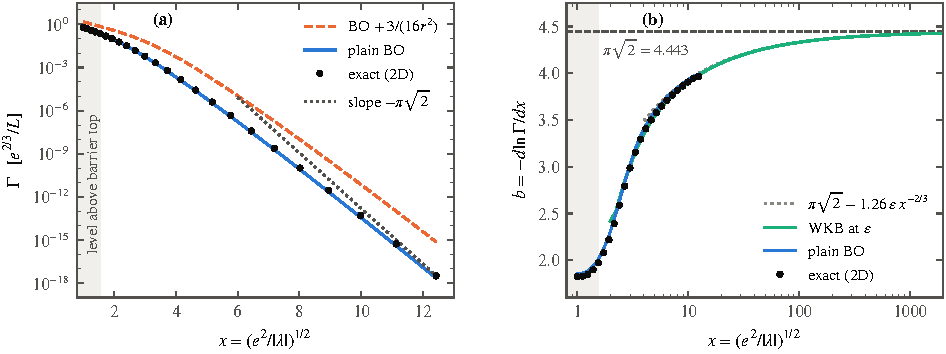
\includegraphics[width=\textwidth]{rep_v11_abelian_width}
\caption{Resonance of the abelian Higgs zero-mode problem against $x=(e^2/|\lambda|)^{1/2}$ (units $e=1$).
(a)~Width $\Gamma$ of the exact two-dimensional problem (points), of the plain Born--Oppenheimer model~(\ref{eq:v11-ab-UBO}) (solid) and of the model with the diagonal term $3/(16r^2)$ (dashed); dotted: slope $-\pi\sqrt2$ of the deep-well law through the last point.
(b)~Local exponent $b=-d\ln\Gamma/dx$: exact (points), plain Born--Oppenheimer (blue), and the WKB action of the Langer-corrected Born--Oppenheimer barrier at the computed energy (green), continued beyond $x=12.4$ with the extrapolated energy $\varepsilon_0=1.9026$; dotted: the leading-order form~(\ref{eq:v11-ab-Seps}); dashed: the deep-well value $\pi\sqrt2$. %
Shaded: the level lies above the barrier top.} %
\label{fig:v11-ab-width}
\end{figure}

\paragraph{Thresholds.}
A box that exists for $N$ light-crossing times keeps the resonance with probability $e^{-\Gamma N}$, and the threshold $\Lambda_c(N)$ solves $\Gamma N=\ln2$; we interpolate $\ln\Gamma$ by a cubic spline in $x$ and include a tenth of the difference from linear interpolation in the uncertainty.
Table~\ref{tab:v11-ab-thresholds} and Fig.~\ref{fig:v11-ab-threshold} give the results for $e=1$: $\Lambda_c=-0.2295$, $-0.09138$, $-0.05252$ and $-0.03123$ for $N=10$, $300$, $10^4$ and $10^6$, with uncertainties of at most $4\times10^{-5}$. %
For general $e$ the condition reads $e^{2/3}F(\Lambda_c)N=\ln2$, and $\lambda_c=e^2\Lambda_c$.

With a constant prefactor, $\Gamma=A\exp(-\pi\sqrt2\,x)$ gives $1/|\Lambda_c|^{1/2}=[\ln N+\ln(A/\ln2)]/(\pi\sqrt2)$, linear in $\ln N$ with slope $1/(\pi\sqrt2)$, so that $|\Lambda_c|^{1/2}\ln N\to\pi\sqrt2$ with corrections of order $1/\ln N$.
With Eq.~(\ref{eq:v11-ab-Seps}), $\ln(N/\ln2)=S(\varepsilon,x_c)+\ln T+O(1)$ gives $|\Lambda_c|^{1/2}\ln N=\pi\sqrt2\,[1-O((\ln N)^{-2/3})]$: the energy of the level adds a slower correction, which dominates as $N\to\infty$.
The computed thresholds approach the limit slowly: $|\Lambda_c|^{1/2}\ln N$ rises from $1.10$ at $N=10$ to $3.16$ at $N=10^{16}$, with local slope $d|\Lambda_c|^{1/2}/d(1/\ln N)$ from $0.52$ to $2.52$, and a straight line through $N=10^4$--$10^{16}$ has slope $1.76$ and intercept $+0.044$ (largest residual $0.006$). %
A constant prefactor as large as the effective prefactors of Table~\ref{tab:v11-ab-widths} would also give a slow approach, so these numbers describe the thresholds without separating the two corrections; the evidence for the energy term is the local exponent $b$ and its agreement with $dS(\varepsilon)/dx$. %
The continuation with the WKB action at the computed energy, anchored to the exact width at $x=12.4$, gives $|\Lambda_c|^{1/2}\ln N=3.75$, $3.98$ and $4.21$ at $N=10^{50}$, $10^{100}$ and $10^{300}$. %
This limit is a property of the abelian model, in which $\Gamma$ vanishes at $\Lambda=0$ because the potential $\frac32er$ then confines; for the Standard Model zero-mode model, which contains $\Delta V$, only the logarithmic dependence on the duration over the computed range is claimed (Sec.~\ref{sec:v11-static-box}).

At the Standard Model slope $\sigma_0=1.31$ ($e=0.8733$) the thresholds are $\lambda_c=-0.182$, $-0.071$, $-0.041$ and $-0.024$ for $N=10$, $300$, $10^4$ and $10^6$. %
The value at $N=300$, $\abelLamcSM$, is six times deeper than the static-box threshold $\lamc(300)=\lcAthree$ of the Standard Model (Sec.~\ref{sec:v11-static-box}). %
The abelian model lacks the two ingredients that make the Standard Model barrier more transparent: the one-loop energy $\Delta V$ of the non-zero modes, which roughly halves the barrier above the level (Sec.~\ref{sec:rb-size}), and the SU(2) zero-mode energy, through which the zero-point energy of the reduced Standard Model model rises with slope $\zpSlopeLo$--$\zpSlopeHi$ at $r=1$--$5$ instead of $\sigma_0$ (Sec.~\ref{sec:v11-static-box}). %
At $\lambda=-0.010$ the barrier of Eq.~(\ref{eq:v11-ab-UBO}) rises $3.25/L$ above the level at this slope, against $1.57/L$ in the reduced Standard Model model without $\Delta V$ and $0.72/L$ with it (Sec.~\ref{sec:rb-size}). %
Accordingly the abelian width there is $\Gamma=6.01\times10^{-12}/L$, against $\Gamma_{\rm 2D}=4.15\times10^{-4}/L$ in the reduced Standard Model model at fixed couplings (Table~\ref{tab:rb-widths}); its exponent $-\ln(\Gamma L\,e^{-2/3})=25.75$ lies well below the deep-well value $38.80$. %

\begin{table}[t]
\centering
\caption{Thresholds $\Gamma N=\ln2$ of the abelian Higgs model in units $e=1$, $\Lambda_c=\lambda_c/e^2$: exact two-dimensional widths (uncertainty at most $4\times10^{-5}$ in $\Lambda_c$), plain Born--Oppenheimer (BO) and BO with the diagonal term (BOD), the combination $|\Lambda_c|^{1/2}\ln N$ with its local slope against $1/\ln N$, and $\lambda_c$ at the Standard Model slope $\sigma_0=1.31$ ($e=0.8733$). In the deep-well limit $|\Lambda_c|^{1/2}\ln N\to\pi\sqrt2=4.443$.} %
\label{tab:v11-ab-thresholds}
\small
\begin{tabular}{@{}ccccccc@{}}
\toprule
$N$ & $\Lambda_c$ & $\Lambda_c^{\rm BO}$ & $\Lambda_c^{\rm BOD}$ & $|\Lambda_c|^{1/2}\ln N$ & $d|\Lambda_c|^{1/2}/d(1/\ln N)$ & $\lambda_c$ ($e=0.8733$) \\ %
\midrule
$10$ & $-0.22952$ & $-0.2315$ & $-0.1139$ & $1.103$ & $0.52$ & $-0.1818$ \\ %
$300$ & $-0.09138$ & $-0.0927$ & $-0.0539$ & $1.724$ & $0.94$ & $-0.0709$ \\ %
$10^{4}$ & $-0.05252$ & $-0.0533$ & $-0.0338$ & $2.111$ & $1.29$ & $-0.0405$ \\ %
$10^{6}$ & $-0.03123$ & $-0.0317$ & $-0.0216$ & $2.441$ & $1.64$ & $-0.0240$ \\ %
$10^{8}$ & $-0.02098$ & $-0.0213$ & $-0.0152$ & $2.668$ & $1.90$ & --- \\ %
$10^{10}$ & $-0.01517$ & $-0.0154$ & $-0.0114$ & $2.836$ & $2.10$ & --- \\ %
$10^{12}$ & $-0.01152$ & $-0.0117$ & $-0.0089$ & $2.966$ & $2.27$ & --- \\ %
$10^{14}$ & $-0.00908$ & $-0.0092$ & $-0.0071$ & $3.072$ & $2.40$ & --- \\ %
$10^{16}$ & $-0.00735$ & $-0.0075$ & --- & $3.159$ & $2.52$ & --- \\ %
\bottomrule
\end{tabular}
\end{table}

\begin{figure}[t]
\centering
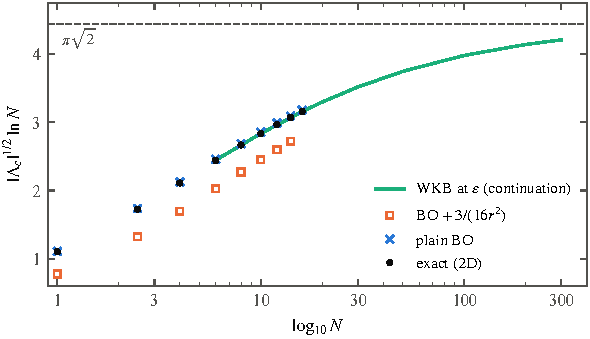
\includegraphics[width=0.62\textwidth]{rep_v11_abelian_threshold}
\caption{Thresholds $\Gamma N=\ln2$ of the abelian Higgs model: $|\Lambda_c|^{1/2}\ln N$ against $\log_{10}N$ for the exact two-dimensional widths (points), the plain Born--Oppenheimer model (crosses) and the model with the diagonal term $3/(16r^2)$ (squares), and the continuation with the WKB action of the Langer-corrected Born--Oppenheimer barrier at the computed energy, anchored to the exact width at $x=12.4$ (line). The deep-well limit $\pi\sqrt2$ (dashed) is approached only as $(\ln N)^{-2/3}$.} %
\label{fig:v11-ab-threshold}
\end{figure}

\paragraph{Accuracy of the Born--Oppenheimer approximation.}
The diagonal BO term follows from $\chi_0$.
With $\partial_\omega\chi_0=\bigl(\frac{3}{4\omega}-\frac{w^2}{2}\bigr)\chi_0$ and $\langle w^2/2\rangle=3/(4\omega)$,
\begin{equation}
\langle\partial_\omega\chi_0|\partial_\omega\chi_0\rangle={\rm Var}\Bigl(\frac{w^2}{2}\Bigr)=\frac14\sum_{i=1}^3{\rm Var}\bigl(w_i^2\bigr)=\frac14\cdot3\cdot2\Bigl(\frac{1}{2\omega}\Bigr)^2=\frac{3}{8\omega^2},
\label{eq:v11-ab-var}
\end{equation}
and with $\partial_r=e\,\partial_\omega$
\begin{equation}
\tfrac12\,\langle\partial_r\chi_0|\partial_r\chi_0\rangle=\frac12\,e^2\,\frac{3}{8e^2r^2}=\frac{3}{16r^2},
\label{eq:v11-ab-diag}
\end{equation}
independent of $e$.
This is the Born--Huang term of the $\bm w$ motion, $B_w$ of Eq.~(\ref{eq:rb-BH}), which in the Standard Model takes this form at small $r$ [Eq.~(\ref{eq:rb-Bw})] and in the abelian model has it at every $r$.
The function $\partial_\omega\chi_0$ is proportional to the first radial excitation $\chi_1$ of the s-wave oscillator, so that the diagonal term is $\frac12A^2$, where $A=\langle\chi_1|\partial_r\chi_0\rangle=(3/8)^{1/2}/r$ is the only non-adiabatic coupling of the ground channel, to a channel $2er$ higher.
Adding Eq.~(\ref{eq:v11-ab-diag}) to Eq.~(\ref{eq:v11-ab-UBO}) gives $U_{\rm BOD}=\frac32er+1/(16r^2)+\lambda r^4/4$, with the Frobenius exponent $a=1.1124$ in place of $1/2$. %
For a bound ground state the BO energy without the diagonal term is a lower bound and with it an upper bound; the computed resonance energies obey $\varepsilon_{\rm BO}<\varepsilon<\varepsilon_{\rm BOD}$ at every $\Lambda$. %

The plain BO model places the level $0.096$--$0.103$ below the exact one and gives widths within $\abelBOdev$: $\Gamma_{\rm BO}/\Gamma$ falls from $1.02$ at $\Lambda=-1$ through $0.85$ at $\Lambda=-0.030$ to $0.72$ at $\Lambda=-0.0065$, and $b_{\rm BO}-b=+0.02$ to $+0.04$ (Table~\ref{tab:v11-ab-widths}, Fig.~\ref{fig:v11-ab-width}). %
The slow drift of $\Gamma_{\rm BO}/\Gamma$ follows from the energy error through Eq.~(\ref{eq:v11-ab-Seps}), $\Delta S\approx3.78\times0.10\,x^{1/3}$, and the BO thresholds lie within $1.5\%$ of the exact ones (Table~\ref{tab:v11-ab-thresholds}). %
With the diagonal term the level lies $0.50$--$0.65$ too high, the widths are too large by factors of $2.5$ ($\Lambda=-1$) to $233$ ($\Lambda=-0.0065$), $b$ is too low by $0.2$--$0.9$, and the thresholds are $22$--$50\%$ shallower. %
The exact level lies at $13$--$17\%$ of the bracket $[\varepsilon_{\rm BO},\varepsilon_{\rm BOD}]$, so that the non-adiabatic couplings, leading at second order, cancel $83$--$87\%$ of the shift produced by the diagonal term. %
The reason is the absence of a small parameter.
By the scaling~(\ref{eq:v11-ab-scaling}) the $w$ frequency in the well, $er$ at $r\approx e^{-1/3}$, and the energy scale of the $r$ motion are both proportional to $e^{2/3}$, so their ratio does not depend on the coupling; in the well the kinetic energy of the $r$ motion, about $\varepsilon/3$ by the virial theorem for a linear well, is comparable with the gap $2er$, and the second-order energy of the coupling $A$, of order $A^2\langle p_r^2\rangle/(2er)$, is of the same order as $\frac12A^2$.
Only under the barrier, at $r\approx|\Lambda|^{-1/3}$ in units $e=1$, is the $w$ motion fast.
A one-dimensional reduction with the diagonal BO term is therefore unsuitable for quantitative widths, and the plain BO model, or better the BO barrier at the exact energy, is accurate to tens of per cent.

The reduced Standard Model model of Sec.~\ref{rep:h-reduced} solves $r$ and $|\bm w|$ together and does not use the diagonal term for $\bm w$.
Its hypercharge mode also has a frequency that vanishes linearly as $r\to0$, and Sec.~\ref{rep:h-reduced} found the same pattern there: the two-dimensional energy lies at $15.5\%$ of its BO bracket at $\lambda=0$, and nearly all of $B_w$ is spurious (Table~\ref{tab:rb-lam0} and the discussion of the mechanism). %
The abelian model, solved without any reduction, shows that this is a property of a fast mode whose frequency vanishes linearly in the slow coordinate, independent of the approximations of Sec.~\ref{rep:h-reduced}, and that a one-dimensional reduction with that term would overestimate the widths by orders of magnitude.
The SU(2) modes, which the magnetic quartic term keeps stiff at small $r$, enter the reduced model through the conditional Gaussian with the Born--Huang term $B_x\le0.012$ for $r\le3$ (Table~\ref{tab:rb-BH}); the full-dimensional calculation of Secs.~\ref{sec:v18-problem}--\ref{sec:v18-mc} tests that part directly. %

\paragraph{Compactness of the holonomy.}
The truncation treats $\bm w$ as non-compact.
A large gauge transformation shifts each $ew_i$ by $2\pi$, so the configuration space of the constant connections is the fundamental domain $|ew_i|\le\pi$, and near its boundary a charged mode of non-zero momentum becomes as light as the constant mode, where the zero-mode Hamiltonian no longer applies.
In the converged resonance wave functions, inside the radius of the barrier top, the probability that $e|\bm w|$ exceeds $\pi$, an upper bound on the probability that some component leaves the domain, is $1.8$--$2.6\times10^{-3}$ for $e=1$, $5.5$--$8.1\times10^{-4}$ for $e=0.873$ ($8.0\times10^{-4}$ at $\lambda=-0.010$) and $3.2$--$5.9\times10^{-7}$ for $e=0.5$. %
Beyond $e|\bm w|=\pi/2$ it is $23$--$26\%$, $16$--$19\%$ and $1.9$--$2.4\%$; the ranges cover $\Lambda=-1$ to $-0.0065$, with the narrow resonances at the upper ends, and direct calculations at $e=0.873$ reproduce the values obtained by scaling. %
The non-compact treatment therefore affects a probability below $\abelHolonomy$ at the Standard Model slope. %
Its effect on $\Gamma$, through the energy of the level, was not computed; by Eq.~(\ref{eq:v11-ab-Seps}), $\delta\ln\Gamma\approx3.78\,x^{1/3}\,\delta\varepsilon\approx8\,\delta\varepsilon$ at $e=0.873$ and $\lambda=-0.010$, so a level shift of order $10^{-3}$ would change $\Gamma$ at the per-cent level. %
The wave function is, however, not deep inside the domain for $e\approx0.87$--$1$: about a fifth of the probability lies beyond half of it. %

\paragraph{Without the gauge modes.}
For $e\to0$ at fixed $\lambda<0$ the problem is $-\frac12\nabla_\phi^2+\frac\lambda4|\bm\phi|^4$ on the plane, whose potential decreases monotonically from zero: there is no well, no barrier and no quasi-bound state.
Scaling $r\to\mu r$ with $\mu^6=-1/|\lambda|$ maps the inverted quartic to $|\lambda|^{1/3}e^{-i\pi/3}$ times the quartic oscillator $-\frac12\nabla^2+\frac14r^4$, so that every complex-scaled eigenvalue lies on the ray $\arg E=-60^\circ$, with $\Gamma/{\rm Re}\,E=2\sqrt3$ for every $\lambda$.
At $\lambda=-0.03$ the lowest one is $E=0.14457-0.25040\,i$, at $\arg E=-60.000000^\circ$. %
This pole is fixed by the scaling of the inverted quartic and is not a narrow resonance.
In the form~(\ref{eq:v11-ab-Hu}) the reduced potential $-1/(8r^2)+\lambda r^4/4$ is not monotonic: it has a maximum of negative height $-\frac{3}{16}(4|\lambda|)^{1/3}$ at $r=(4|\lambda|)^{-1/6}$.
This maximum is not a barrier, since $-1/(8r^2)$ is the $m=0$ kinetic term of the plane, which the Langer substitution removes; the potential of the problem, $\lambda|\bm\phi|^4/4$, is monotonic.
The narrow resonance of the model is therefore due to the gauge zero modes, as for the gauge zero-mode switch of the Standard Model calculation (Sec.~\ref{sec:v11-kappa}).

\paragraph{What the test establishes.}
\emph{Proved.} The zero-mode problem of the abelian Higgs model reduces exactly to $(r,s)$; its resonance obeys Eq.~(\ref{eq:v11-ab-scaling}); the diagonal BO term is $3/(16r^2)$. %

\emph{Under stated conditions}, in the WKB approximation for the Langer-corrected BO barrier, which is asymptotically exact as $x\to\infty$: the deep-well exponent is $\pi\sqrt2\,x$, and the energy of the level lowers the barrier action by $3.78\,\varepsilon\,x^{1/3}$ at leading order. %

\emph{Found numerically}, with relative precision of order $10^{-8}$ internally and $10^{-6}$ against the independent method at $-0.416\le\Lambda\le-0.0155$ (the blind recalculation of Sec.~\ref{sec:v11-blind-abelian} also covers $\Lambda=-1$ and $-0.01003$): the gauge zero modes alone confine the negative quartic, with widths from $0.61$ to $3.2\times10^{-18}$; the local exponent rises from $1.8$ to $4.0$ and is reproduced by the WKB action of the BO barrier at the computed energy; the plain BO widths lie within $30\%$ of the exact ones, and the widths with the diagonal term are too large by up to $233$; the weight beyond the fundamental domain of the holonomy is below $10^{-3}$ for $e\le0.87$. %

\emph{Expected}, from the WKB continuation: $b=4.28$ and $4.42$ at $x=60$ and $1000$, and the approach of $|\Lambda_c|^{1/2}\ln N$ to $\pi\sqrt2$; these rest on the barrier action at an extrapolated energy, with a prefactor ratio that varies slowly ($0.80$ to $0.757$ over $x=3$--$12.4$). %

\emph{Outside the test.} The model contains no $\Delta V$, no SU(2) modes, no fermions and no cross terms; it tests the mechanism and the WKB form of the width at the resonance energy, whereas the deep-well law with a constant prefactor holds only asymptotically, and it does not test the numbers of the Standard Model, whose threshold at $N=300$ is six times shallower than that of the model at the same zero-point slope. %
It does not test the conditional Gaussian of the SU(2) modes or the DMC shape correction, which the full-dimensional calculation of this section tests, and it omits the compactness of the holonomy and the light charged modes near the boundary of the fundamental domain, whose weight it bounds.
